\chapter{Hybrid Wireless Rural Broadband Networks}
\label{chapter3}
The first testing scenario EMANE was placed under was emulating two wireless, hybrid network topologies that were designed to more effectively deliver broadband to small rural communities.
Since deploying broadband to rural communities can be expensive through traditional methods, wireless distribution topologies have become a popular way of bringing the Internet to these communities.
As was explained, testing wireless networks in hardware is rather expensive, and finding a location that meets the environmental factors of the target rural communities is challenging.
To solve these issues, initial testing can be conducted in EMANE. This allows an understanding of the interactions between the technologies selected to be formed, and do basic validation that the proposed network can feasibly achieve its goal.

\section{Hardware Testbed Network Topologies}
    % Hardware testbed utilized a mmWave backhaul and Ubiquiti LTU radios for the distribution network
        % mmWave and LTU were abstracted using rfPipe in EMANE
    % Allowed for testing throughput and bandwidth characteristics with multiple hosts connected as well as range using simple pathloss models
Both of the network architectures that will be examined in this chapter were eventually set up in hardware.
While these hardware testbeds were being built, emulated EMANE testbeds were also set up.
Both testbeds can be classified by two distinct wireless technologies, the first stage is a mmWave backhaul.
This wireless, high data rate backhaul was intended to replace the traditional wired backhaul, that makes reaching these rural communities so difficult.
The other technology used was Ubiquiti's proprietary LTU protocol.
The LTU leg of the network consisted of the distribution portion of the network and was responsible for bridging the connected houses to the backhaul.
By abstracting both of these technologies into EMANE, testing characteristic behaviors of the network with several hosts was possible.
A pfSense Router was also used in both testbeds to handle all routing requirements.
Thanks to EMANE's hardware in the loop capabilities, the actual pfSense software was used in the experiment emulation testbed.

\subsection{OVERCOME Testbed}
    % Topology
        % (FIGURE\_OVERCOMETopology)
        % Two sets of mmWave backhauls
        % Aggregate at a router in the middle of town
        % Split into 3 radios for distribution to ~30 houses
The first of the two testbeds was located in Turney, Missouri, a small community outside of Kansas City that was not currently covered by any of the Internet Service Providers in the area.
The topology of the network can be seen in Figure~\ref{overcome_topology}.
\begin{figure}[!ht]
    \centering
    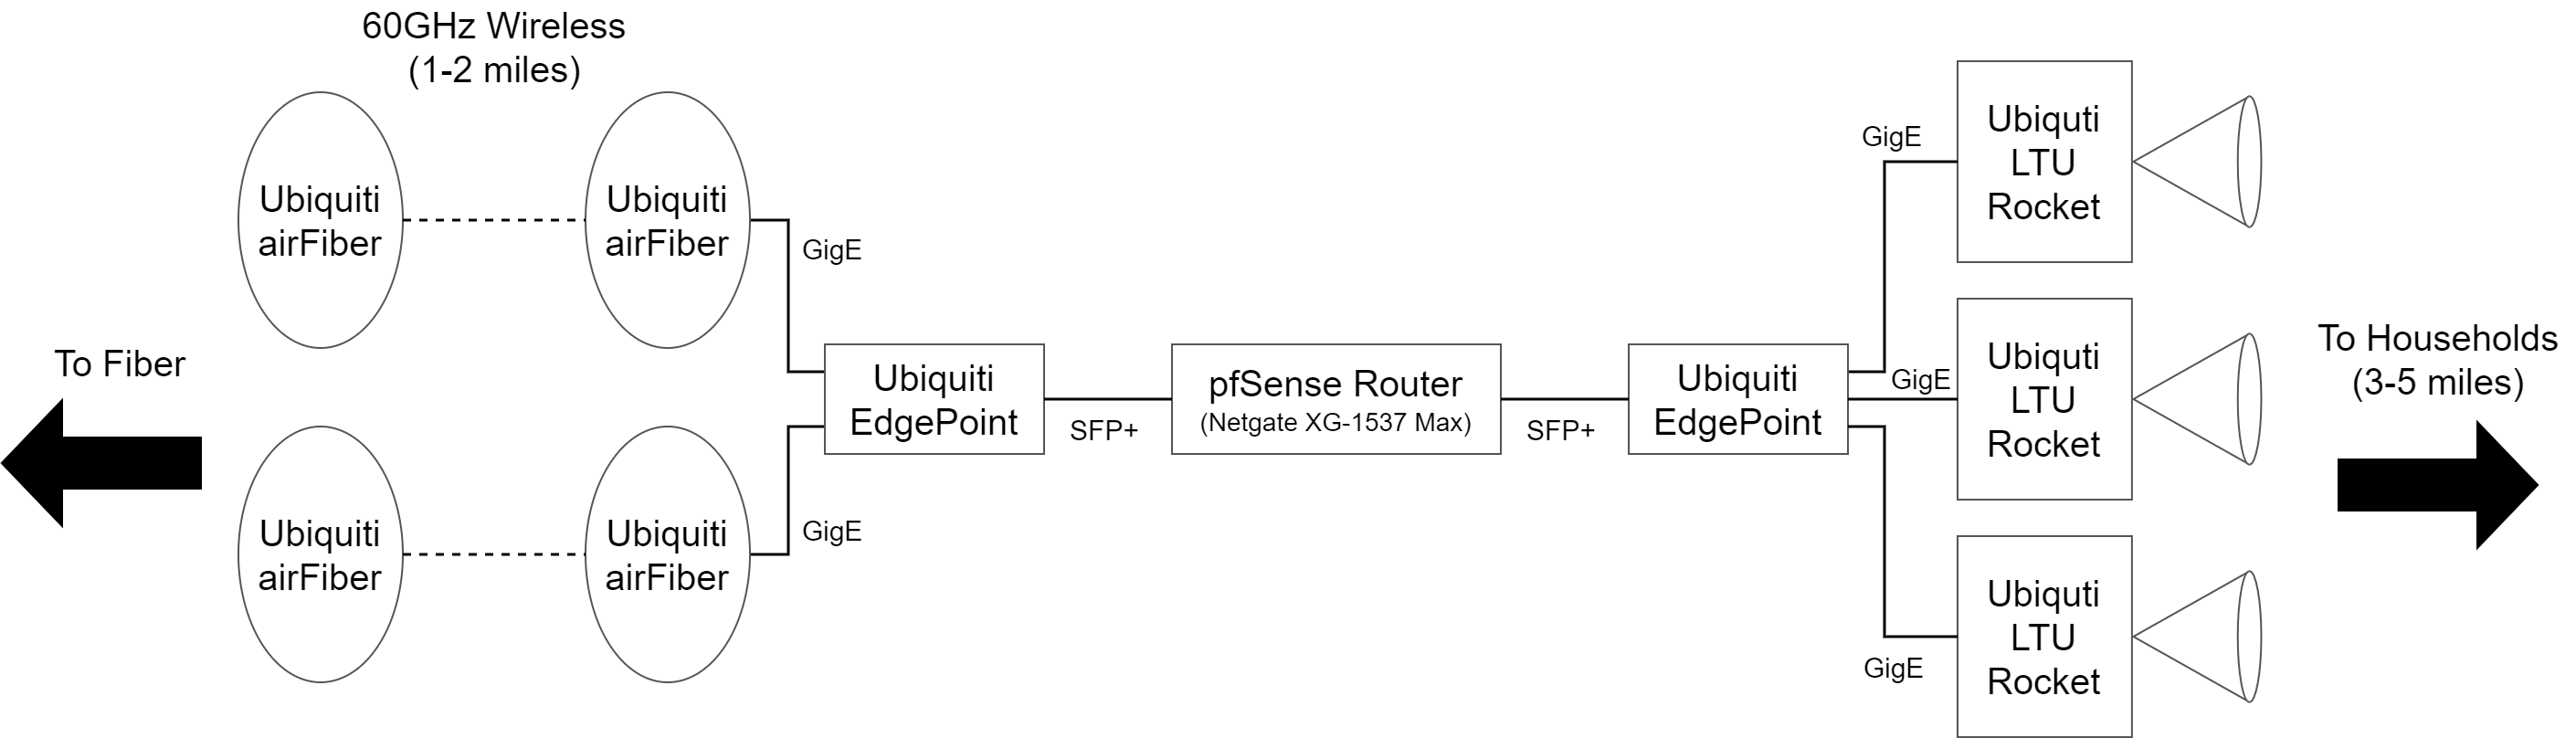
\includegraphics[width=\textwidth,keepaspectratio]{Images/Chpt3/OVERCOME_Topology.png}
    \caption{The network topology of the testbed built as part of Project OVERCOME in Turney, MO.}
    \label{overcome_topology}
\end{figure}
In order to create this topology in EMANE, we first had to understand the major characteristics of the hardware being mimicked.
    % Technologies used
        % Ubiquiti AirFiber, Ubiquiti Edge Switches, Netgate pfSense Router, Ubiquiti LTU Rockets
The mmWave backhaul consisted of four Ubiquiti airFiber 60LR radios.
These two pairs of point-to-point radios acted as the backhaul of the network and carried the traffic from the nearest location with fiber, to the center of the community.
Once arriving at the center of Turney, the traffic was passed through a commercial Netgate XG-1537 Max router running pfSense.
This router was primarily responsible for switching traffic off the ISP's network and onto the last leg of the network to the homes.
The final piece of the network was the LTU leg.
The transmitting radios from the center of town to all the homes were three Ubiquiti LTU Rockets.
These radios connected to an Ubiquiti LTU Pro at each house, which provided Internet connectivity to the user. 

\subsection{ZoomTEL Testbed}
    % Topology
        % (FIGURE\_ZoomTELTopology)
        % Two-hop mmWave backhaul
        % LTE-U distribution network at each hop
        % Distribute to hosts centered around each hop
The second testbed topology was not deployed to an actual location where it would be permanently used, and was instead just tested locally.
The topology of what was tested can be seen in Figure~\ref{zoomtel_topology}.
\begin{figure}[!ht]
    \centering
    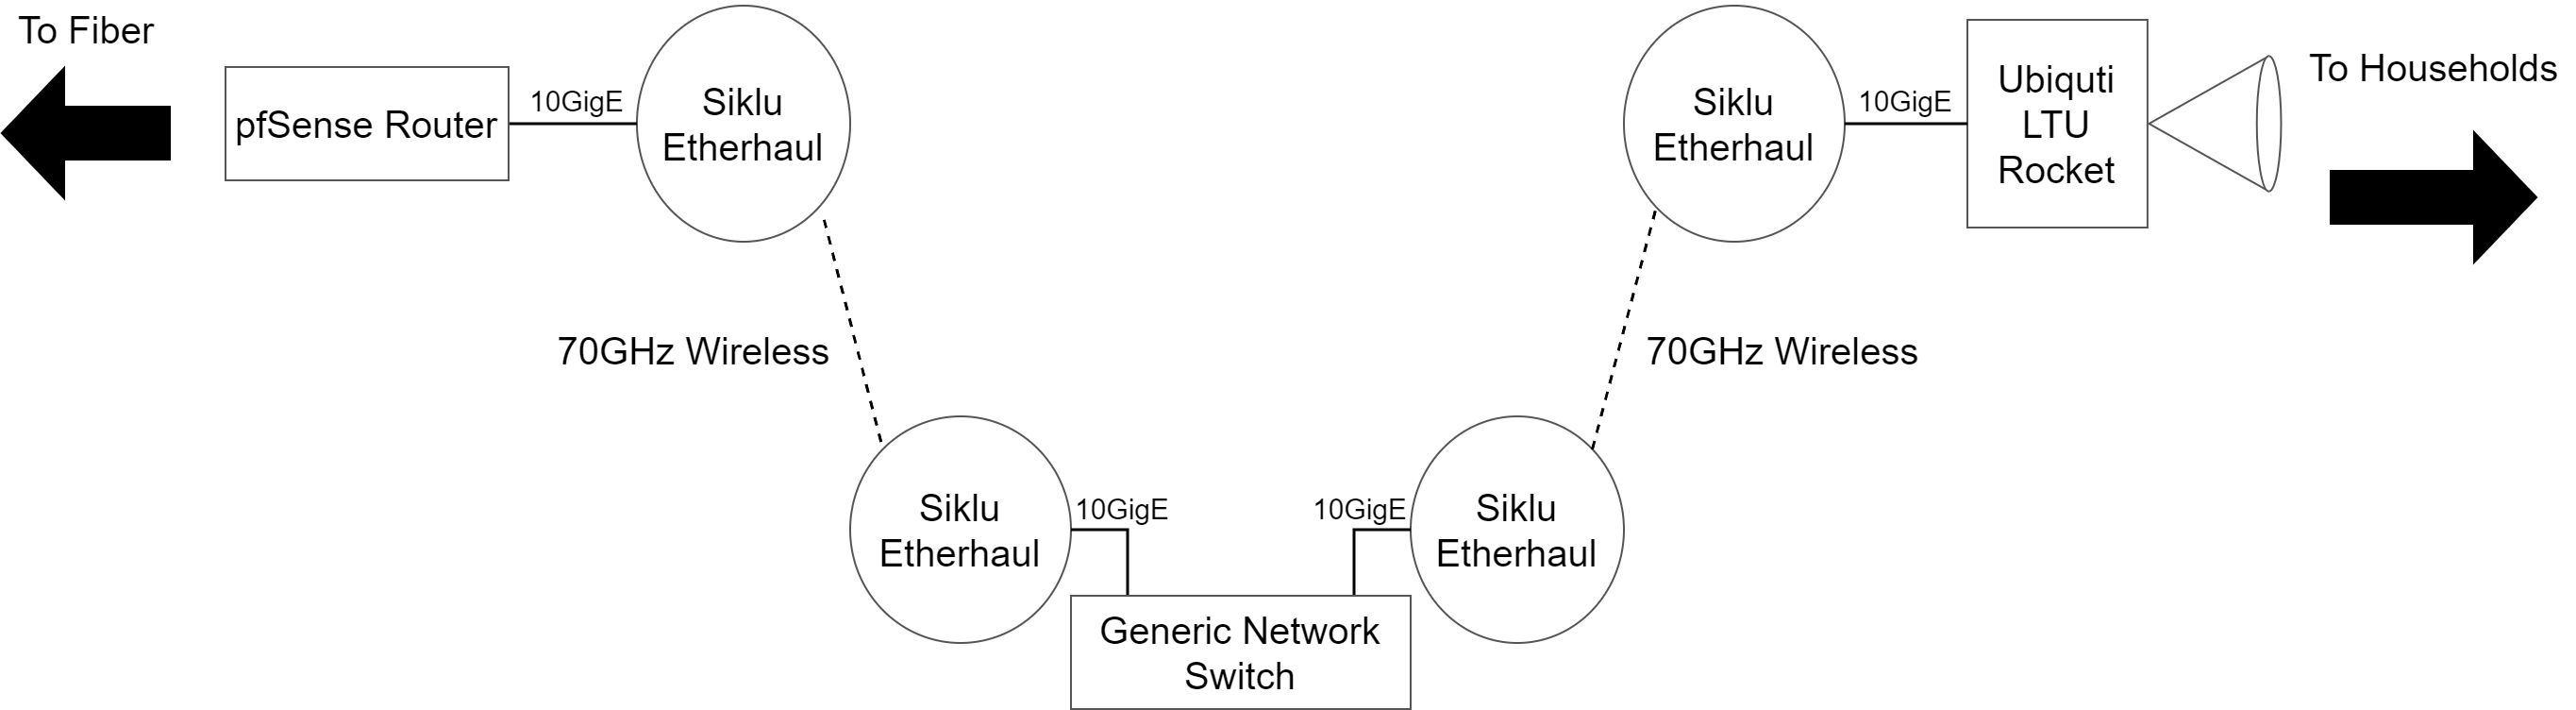
\includegraphics[width=\textwidth,keepaspectratio]{Images/Chpt3/ZoomTEL_Topology.png}
    \caption{The network topology of the experimental testbed built as part of the ZoomTEL project.}
    \label{zoomtel_topology}
\end{figure}
The primary idea behind this network topology, and what makes it differ from the OVERCOME topology, is that the segment shown in Figure~\ref{zoomtel_topology} is intended to be repeated and tiled to create a mesh of backhaul connections.
This would allow the pfSense route at the origin of the mesh to make routing determinations based on the quality of links in the network, and could attempt to solve the issue of the delicate nature of mmWave links, especially when concerning weather systems.
In this thesis only the single segment shown in Figure~\ref{zoomtel_topology} was implemented for testing, but could easily be expanded in EMANE.\par
    % Technologies used
        % Siklu EtherHaul, Ubiquiti network switches, Ubiquiti LTU Rockets
The technologies used in this testbed are similar to the ones in the previous network, but the equipment that implements primarily the mmWave links is different.
In this network, the fiber is directly connected to a pfSense router instead of the backhaul, this allows the special routing functionality that was described.
The hardware network tested in this topology used a generic Dell OptiPlex desktop as the router.
Since the pfSense software is free to use, a commercial solution does not need to be purchased to use it.
All the mmWave links were created using the Siklu Kilo Series EtherHaul 1200, four of which were used.
The LTU link used the same Ubiquiti LTU Rocket as the radio located at the backhaul, but unlike the OVERCOME project, the LTU Lite radios were used as the customer premises equipment (CPE).


\section{Creating the Networks in EMANE}
    % Creating mmWave and LTU in EMANE
        % Use rfPipe to mimic characteristics of mmWave and LTU
            % Bandwidth, delay, throughput, frequency of interest, distance between radios, antenna RX and TX gains
In order to implement the mmWave and LTU wireless technologies into EMANE, the rfPipe model was selected.
Since the primary concern with the emulation testbed was mimicking the general behavior of the network, it was decided the that rfPipe model would work well enough, and a more complex model was not needed.
Table~\ref{mmwave_params} outlines the key configuration parameters that were used to create the mmWave links.
Table~\ref{ltu_params} outlines the same parameters and their selected values for the LTU waveforms.
Since the LTU radios varied between testbeds and the characteristics of the basestation radio and CPE radios were different from each other, values that would most accurately model the average expected behavior were selected.
This could cause some variation in the results, but it was deemed acceptable for the proposed use case.
Most of these parameters were selected based on the datasheets of both radio platforms and the antennas (integrate or external) that were used.
This is information that would be available prior to purchasing hardware to validate a design.
The freespace pathloss model was selected as the effects of multipath were not expected to be a primary concern in the testbeds.\par
\begin{table}[!ht]
\centering
\caption{mmWave Model EMANE Parameters}
\begin{tabular}{lr} 
\hline
\multicolumn{1}{c}{EMANE Parameter} & \multicolumn{1}{c}{Value} \\ 
\hline
Delay & 0.5ms \\
Data Rate & 1Gbps \\
Frequency & 60GHz \\
Channel Width & 500MHz \\
Fixed Antenna Gain & 43dBi \\
Pathloss Model & \multicolumn{1}{l}{Freespace} \\
\hline
\end{tabular}
\label{mmwave_params}
\end{table}
\begin{table}[!ht]
\centering
\caption{Ubiquiti LTU Model EMANE Parameters}
\begin{tabular}{lr} 
\hline
\multicolumn{1}{c}{EMANE Parameter} & \multicolumn{1}{c}{Value} \\ 
\hline
Delay & 2.5ms \\
Data Rate & 200Mbps \\
Frequency & 5.8GHz \\
Channel Width & 20MHz \\
Fixed Antenna Gain & 19.5dBi \\
Pathloss Model & \multicolumn{1}{l}{Freespace} \\
\hline
\end{tabular}
\label{ltu_params}
\end{table}
\begin{figure}[!ht]
    \centering
    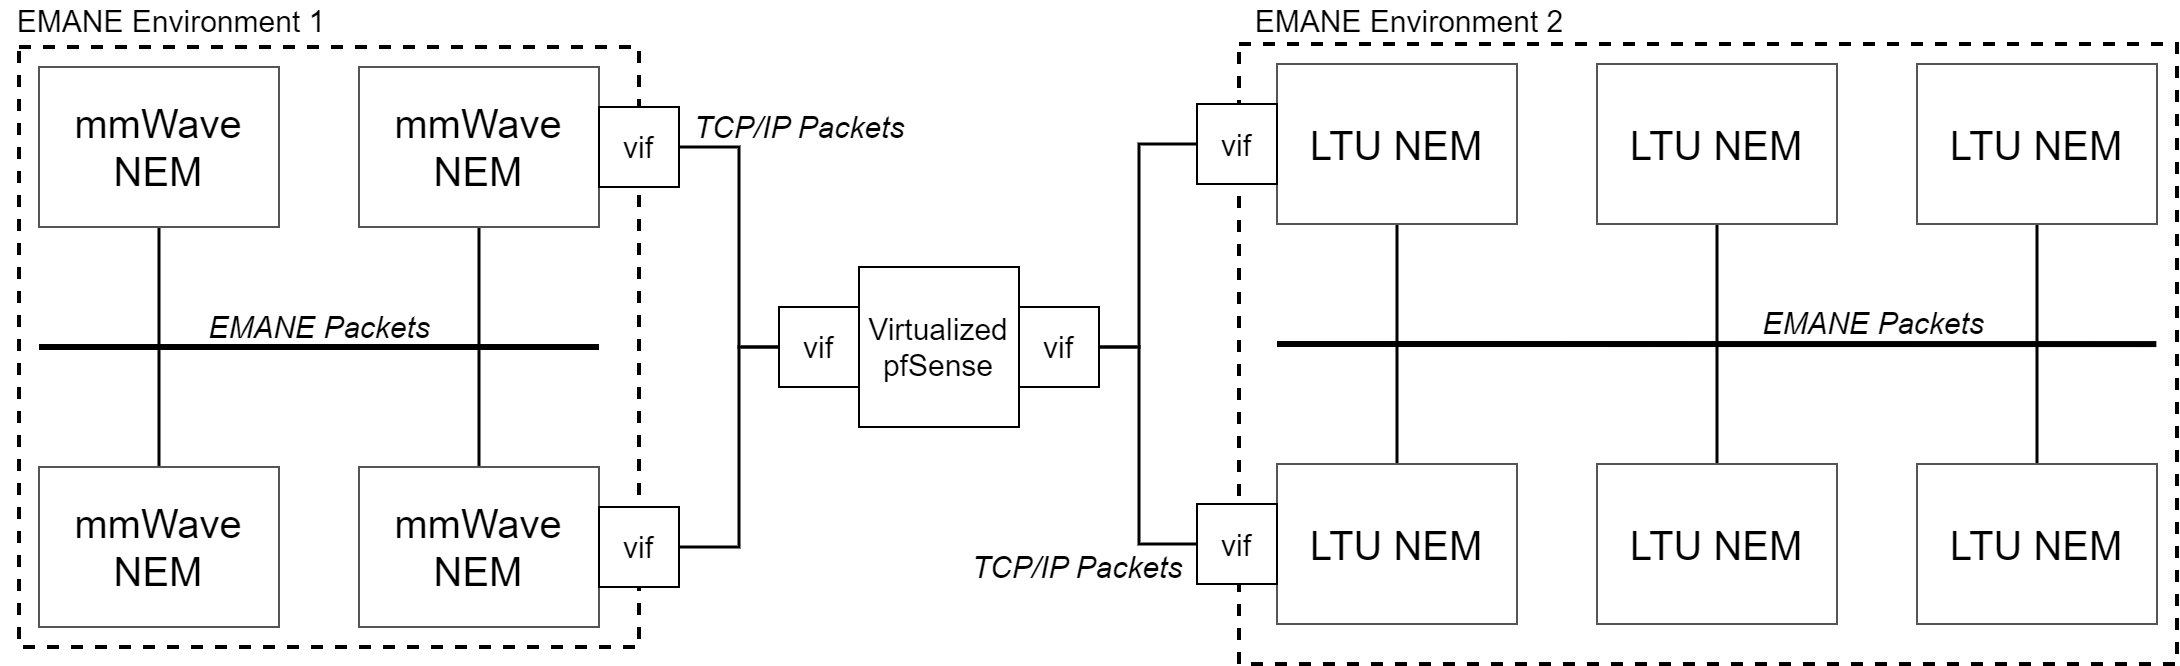
\includegraphics[width=\textwidth,keepaspectratio]{Images/Chpt3/EMANE_OVERCOME.png}
    \caption{The emulation testbed topology corresponding to the OVERCOME project.}
    \label{overcome_emane}
\end{figure}
\begin{figure}[!ht]
    \centering
    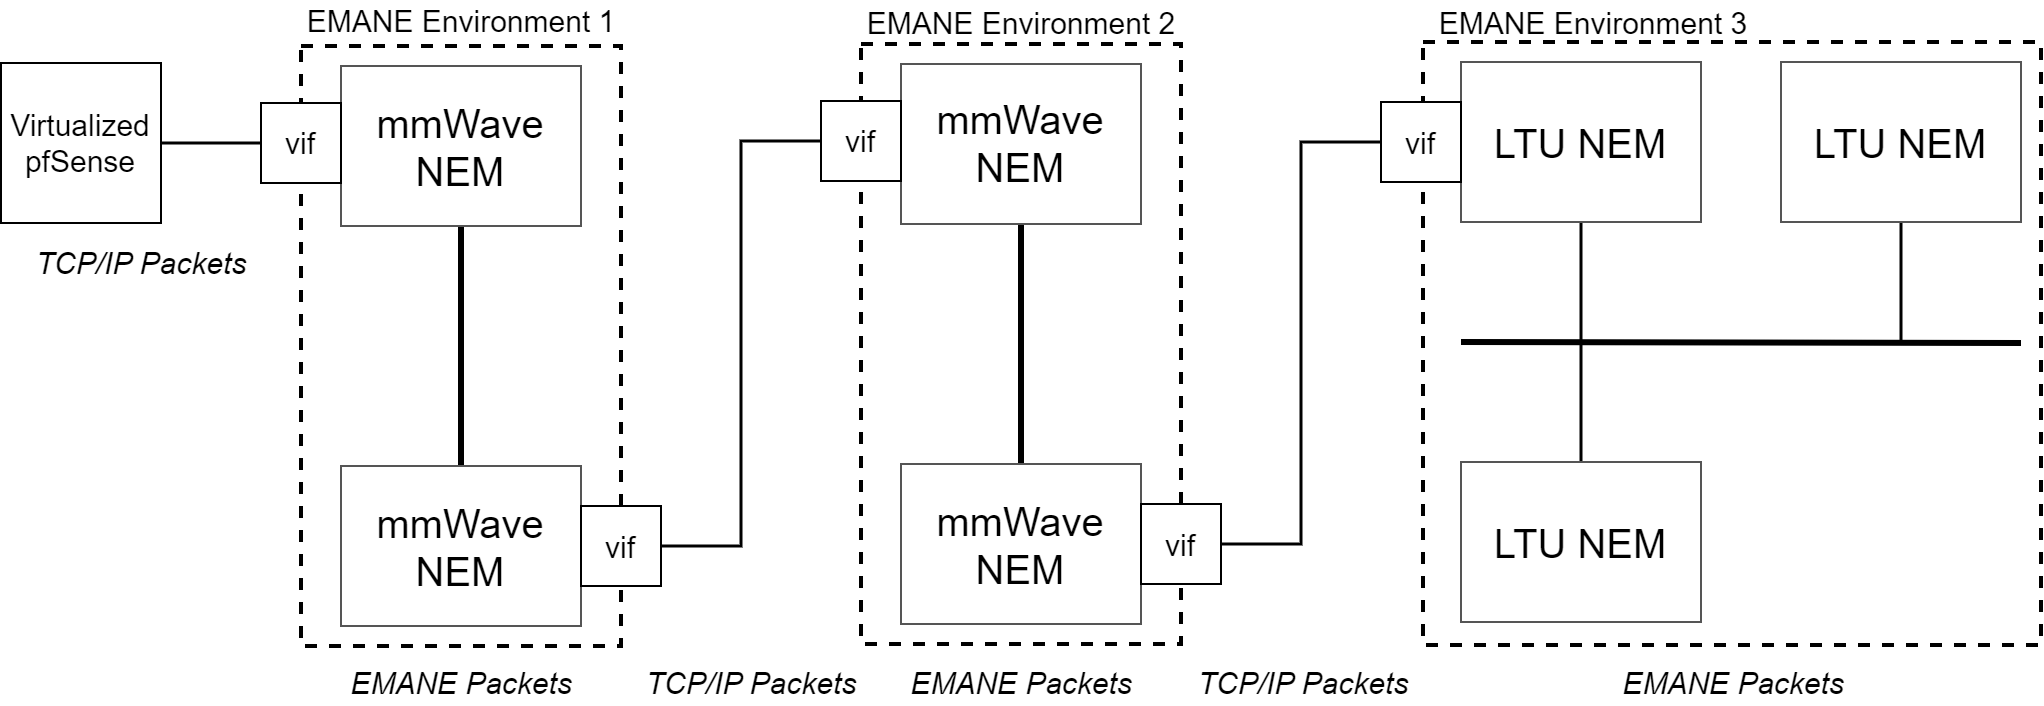
\includegraphics[width=\textwidth,keepaspectratio]{Images/Chpt3/EMANE_ZoomTEL.png}
    \caption{The emulation testbed topology corresponding to the ZoomTEL project.}
    \label{zoomtel_emane}
\end{figure}
With the radio plugins configured in the NEMs, two EMANE environments were created for the OVERCOME testbed, and three EMANE environments were created for the ZoomTEL testbed.
These emulation topologies can be seen in Figure~\ref{overcome_emane} and Figure~\ref{zoomtel_emane}, respectively.
It is important to note that the two individual mmWave links in the ZoomTEL topology are separate EMANE instances.
These could have been put in the same environment as was the case with the OVERCOME testbed, however it was elected to make them entirely separate to allow for more control over the events that were used to effect the operational environment.
If a weather system and its effects on the channel were to be modeled, being able to only impart those effects on a single mmWave link is a very useful ability to have, especially if the testbed was developed further to implement the poor link quality avoidance routing system previously described.\par
    % Interfacing with a real pfSense router in EMANE
        % Use EMANE transport plugins to delivery and receive real TCP/IP packets from a virtualized router
        % Performance implications of using a virtualized router vs. the real hardware router?
            % (No, there was such limited traffic that the hardware router was never pushed beyond a few percent usage, and the virtual router never bottlenecked)
In both testbeds, a pfSense router is virtualized and inserted into the emulation loop.
This was initially a difficult process as understanding exactly how the transports needed to be configured to properly pass the TCP/IP traffic to and from the router to emulator was not clear in the documentation.
Several portions of the example configurations use a transport plugin scheme that is later recommended to not be used, causing lots of confusion.
Eventually a tutorial~\cite{letce2_git} and a forum post~\cite{issues_git} were found that detailed exactly how to connect a virtual machine to a NEM container.
The process primarily relies on creating an additional pair of virtual network interfaces that connect the LXC to the host machine, and having VirtualBox bridge this interface.
Since this new interface is not a part of EMANE directly, and therefore not a member of any routing schemes, manual routes needed to be configured so the LXC would properly forward the packets to and from EMANE.
This is an example of the code that was used to add these manual routes in the ZoomTEL testbed:
\begin{minted}[fontsize=\small, breaklines]{Bash}
#!/bin/bash -
ip route add 10.150.2.0/24 via 10.100.1.2
ip route add 10.100.2.0/24 via 10.100.1.2
ip route add 10.150.3.0/24 via 10.100.1.2
ip route add 10.200.3.0/24 via 10.100.1.2
\end{minted}
This script would run on startup of the initial mmWave LXC node and add routes to the second mmWave emulation network, the LTU network, and the external TCP/IP networks bridging the EMANE instances.\par
One of the important factors taken into consideration when virtualizing pfSense, was if the virtualization of the router software would have performance impacts on the network.
The expectation was that there would not be any major impacts since pfSense is a very lightweight program and is often virtualized in production environments.
For reference, the pfSense router running in production in the OVERCOME project connecting 30 households to the Internet was never recorded at more than a few percent CPU usage.
Similarly, the virtual pfSense router never reached above 5\% CPU usage and the router never indicated it was dropping packets due to computational overload.

\section{Hardware Results versus Emulation Results}
Having built the emulation testbeds, it was time to use them for testing.
Since the hardware testbeds were already in the process of being built, data could be used off the hardware testbed to determine the legitimacy of results produced by EMANE.
If the results showed that the key values like data throughput and latency were accurate, EMANE could be used as a development environment, as detailed in Chapter~\ref{chapter4}.\par
In order to get the relevant data from EMANE, tools like \textit{iperf3} and \textit{ping} were used for generating and measuring traffic.
The \textit{MGEN} utility was also used, and is an open-source tool designed by the Naval Research Lab.
It can be used to generate and log a variety of TCP/IP and UDP/IP traffic and can be used to script traffic behaviors to create repeatable experiments.
An example of an \textit{iperf3} test can be seen in Figure~\ref{iperf_test}
\begin{figure}[!ht]
    \centering
    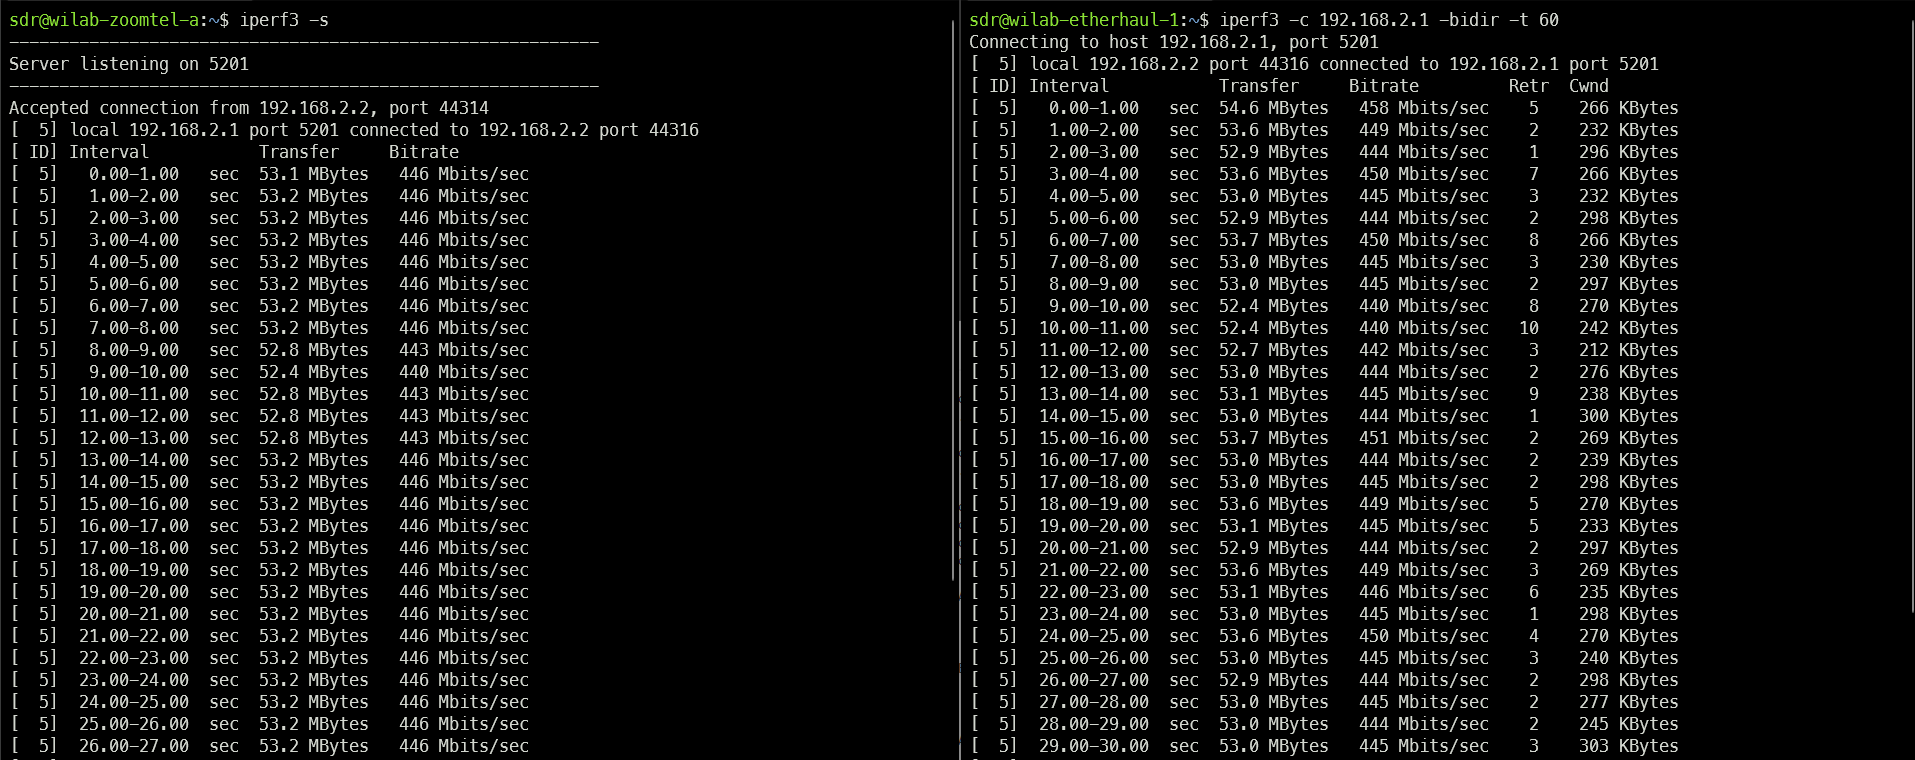
\includegraphics[width=\textwidth,keepaspectratio]{Images/Chpt3/ThroughputTest.png}
    \caption{The console output of an \textit{iperf3} test used to find the throughput for part of the ZoomTEL EMANE testbed.}
    \label{iperf_test}
\end{figure}
The ZoomTEL hardware testbed also used the \textit{iperf3} utility for testing.
The following command was used for running a test on the client:
\begin{minted}[fontsize=\small, breaklines]{Bash}
    iperf3 -c <server ip address> -bidir -t 60
\end{minted}
This command sets the destination of the server (the node being transmitted to) with the "-c" flag.
The "-bidir" flag indicates the test should be run in bidirectional mode so that both the throughput of the uplink and downlink can be measured.
The final flag "-t 60" indicates that the test should run for 60 seconds. This is to ensure a stable enough average is measured since the total throughput can have slight fluctuations.\par
The OVERCOME testbed utilized several tools for recording data.
Throughput and latency tests were measured via the website \textit{speedtest.net}.
This tool was used by the engineers at the Internet Service Provider that installed the equipment at the users home, and the aggregate data was found by taking an average of all results.
Users that lived closer to the center of town had better results, but this was offset in the average by houses further away.
Table~\ref{chpt3_results} shows the average results from all three environments for comparison.\par

\begin{table}
\centering
\caption{Latency and throughput measurements from the Projects OVERCOME, ZoomTEL, and EMANE testbeds.}
\begin{adjustbox}{width=\textwidth, center=\textwidth}
    \begin{tabular}{l|cccc}
    \multicolumn{1}{c|}{} & Throughput (Upload) & Throughput (Download) & \multicolumn{1}{l}{Total Throughput} & Latency \\ 
    \hline
    OVERCOME & 62 Mbps & 275 Mbps & 337Mbps & 6ms \\
    ZoomTEL & 87 Mbps & 87 Mbps & 174Mbps & 5.5ms \\
    EMANE & 96.6 Mbps & 96.7 Mbps & 193.2Mbps & 10ms
    \end{tabular}
\end{adjustbox}
\label{chpt3_results}
\end{table}

There are several discrepancies in the data to address.
These discrepancies do not necessarily imply the EMANE model is unreliable, but it does mean that further refinement and testing should be conducted to ensure accuracy.
Without conducting this further verification, EMANE can not be used on its own for testing as the results can not be fully trusted.\par
The first point of interest is the difference in total throughput between OVERCOME and EMANE.
OVERCOME has a much higher total throughput than EMANE, but this is likely attributed to inaccurate configuration of the CPE devices abstracted in EMANE.
The OVERCOME hardware testbed used higher end LTU radios as CPE and the configuration of the LTU model in EMANE was aligned more with the inexpensive LTU units used in the ZoomTEL testbed.
This is why the results from ZoomTEL and EMANE are much similar.
The uneven speeds in the OVERCOME testbed were a design decision made to allow homes to have higher download speeds.
This asymmetric behavior could not be modeled in EMANE as the generic rfPipe model does not support this functionality.
The latency differences between EMANE and the hardware testbeds is possibly attributed to the packet completion rate curves for the rfPipe models.
These curves may not have been modified enough from the baseline to line up with the actual expected behavior.
Another possibility is the delay parameters not being configured properly.
The values chosen were rather conservative estimates and may have been too high to properly model the accurate behavior of the hardware wireless signal.\par
Looking at the throughput and latency of the rfPipe model is not necessarily enough to declare that rfPipe is fully accurate to a hardware model as factors like power and noise calculations should be verified as well.
Additionally, since EMANE models are highly configurable, any given configuration would also need to be subjected to some level of scrutiny to ensure it is accurate enough for the intended use case.

\section{Chapter Summary}
This chapter outlines how EMANE was used to create digital models of two separate wireless hybrid network topologies that were designed with the intention of delivering broadband to harder to service areas.
The architectures of both testbeds were detailed and the hardware equipment being modeled was outlined.
We then explained the parameters in EMANE that were selected in order to mimic the behavior of the hardware radios. Two rfPipe models were created, one for mmWave and one for LTU.
After building an extensive enough understanding of the transport models within EMANE, a virtual pfSense router was also brought into the loop to create additional accuracies.
The chapter finishes off by showing throughput and latency measurements taken on all testbeds and comparing them.
The results are similar enough that the emulator could be used for initial testing in place of the hardware testbed, but the discrepancies show there is room for further refinement of the emulation model.
Using a more custom model besides rfPipe could also result in better results, but this new model would need to be vigorously tested to ensure its validity.